\documentclass{rapport}
\usepackage{lipsum}
\usepackage{gensymb}
\usepackage{float}
\usepackage{graphicx} % Required for inserting images
\usepackage{amsthm} 
\usepackage{amssymb}
\usepackage{cancel}
\usepackage{polynom}

\usepackage{enumitem}
\usepackage[most, theorems]{tcolorbox}
\usepackage{xcolor}
%\usepackage[italian]{babel} % lingua italiana

%\usepackage[utf8]{inputenc}
\usepackage{pgfplots}
\pgfplotsset{compat=1.18}

\usepackage{tikz}
\newcommand*\circled[2][]{%
  \tikz[baseline=(char.base)]{
    \node[shape=circle,draw=#1,inner sep=1pt] (char) {$\displaystyle #2$};
  }%
}
\usetikzlibrary{patterns}

\usetikzlibrary{arrows.meta}
\usetikzlibrary{matrix, positioning}

\newtcbtheorem{teorema}{Teorema}{
  colback=blue!5!white,
  colframe=blue!75!black,
  enhanced,
  fonttitle=\bfseries,
}{theo}

\newtcbtheorem{definizione}{Definizione}{
    colback=green!5!white, 
    colframe=green!75!black, 
    enhanced,
    fonttitle=\bfseries,
}{def}

\newtcbtheorem{esercizio}{Esercizio}{
    colback=red!5!white, 
    colframe=red!75!black, 
   enhanced,
  fonttitle=\bfseries,
}{es}

\newtcbtheorem{corollario}{Corollario}{
    colback=pink!5!white, 
    colframe=pink!75!black, 
    enhanced,
  fonttitle=\bfseries,
}{corr}

\newtcbtheorem{esempio}{Esempio}{
    colback=purple!5!white, 
    colframe=purple!75!black, 
    enhanced,
  fonttitle=\bfseries,
}{esem}

% \newtheorem{theorem}{Teorema}
% \newtheorem{proposition}[theorem]{Proposizione}
% \newtheorem{corollary}[theorem]{Corollario}
% \newtheorem{lemma}[theorem]{Lemma}

% \theoremstyle{definition}
% \newtheorem{definition}[theorem]{Definizione}
% \newtheorem{axiom}[theorem]{Assioma}
% \newtheorem{example}[theorem]{Esempio}

% \theoremstyle{remark}
% \newtheorem{remark}[theorem]{Remark}
% \newtheorem{note}[theorem]{Note}
\def\mathunderline#1#2{\color{#1}\underline{{\color{black}#2}}\color{black}}
\newcommand{\mathrect}[2]{%
  \fcolorbox{#1}{white}{\strut$\displaystyle #2$}%
}

\title{DataBase} %title of the file

\begin{document}

%----------- Report information ---------

\logo{logos/logo.jpg}
\uni{\textbf{Università degli Studi di Padova}}
\ttitle{Analisi 1} %title of the file
\subject{Analisi 1} % Subject name
\topic{Analisi 1} % Topic name

\students{Alex Gasparini} % information related to the students

%----------- Init -------------------
        
\buildmargins % display margins
\buildcover % create the front cover of the document
\toc % creates the table of contents

%------------ Report body ----------------



\section{Vettori}
\addcontentsline{toc}{subsection}{Vettori}

Come prima attività del corso andiamo a fare un ripasso dei vettori perchè ci serviranno per estendere tutto quello che abbiamo visto ad analisi 1 a più dimensioni, tipicamente in 2d o 3d. 

Ricordiamo un vettore è una collezione di $n$ elementi, per questo sono parte dell'insieme $\mathbb{R}^n$. Per semplicità in questo corso indicheremo con una lineetta sotto quando parliamo di vettori (es: $\underline{x}$) mentre per i scalari indichiamo solo la lettera (es: $x$). I vettori li possiamo rappresentare numericamente in verticale o orizzontale

\[
\underline{x}=\begin{pmatrix} x_1 \\ x_2 \\ \vdots \\ x_n \end{pmatrix} \quad  \quad \underline{y} =  \begin{pmatrix} y_1 & y_2 & \dots & y_n \end{pmatrix}
\]

Le notazioni sono equivalenti. Per i vettori 2D e 3D li possiamo rappresentare rispettivamente nel piano cartesiano e nello spazio euclideo e li possiamo indicare come delle freccie che partono dall'origine fino al punto delle coordinate del vettore.

\vspace{0.2cm}

\noindent
% --- PRIMO GRAFICO: PIANO CARTESIANO (2D) ---
\begin{minipage}[t]{0.48\textwidth}
  \centering
  \textbf{\small Piano Cartesiano (2D)}\\[4pt]
  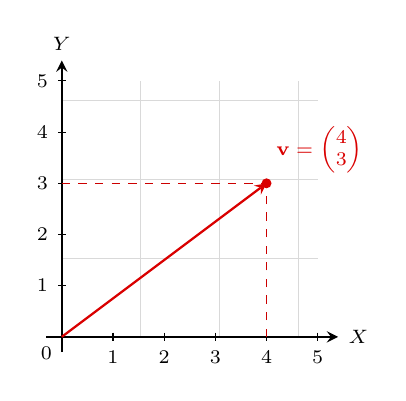
\begin{tikzpicture}[
      >=stealth,
      x=0.65cm, y=0.65cm,
      lbl/.style={font=\scriptsize},
      vec2d/.style={thick, ->, red!85!black},
      dash_red/.style={dashed, thin, red!80!black}
    ]
    % Griglia
    \draw[lightgray!60, very thin] (0,0) grid (5,5);

    % Assi
    \draw[thick, ->] (-0.3,0) -- (5.4,0) node[anchor=west, lbl] {$X$};
    \draw[thick, ->] (0,-0.3) -- (0,5.4) node[anchor=south, lbl] {$Y$};

    % Tacche e numeri
    \foreach \x in {1,...,5}
      \draw (\x, 0.08) -- (\x, -0.08) node[anchor=north, lbl] {\x};
    \foreach \y in {1,...,5}
      \draw (0.08, \y) -- (-0.08, \y) node[anchor=east, lbl] {\y};
    \node[lbl, anchor=north east] at (0,0) {0};

    % Proiezioni
    \coordinate (P2D) at (4,3);
    \draw[dash_red] (4,0) -- (P2D);
    \draw[dash_red] (0,3) -- (P2D);

    % Vettore e punto P
    \draw[vec2d] (0,0) -- (P2D);
    \fill[red!85!black] (P2D) circle (1.8pt);
    \node[lbl, text=red!85!black, anchor=south west] at (P2D) {$\mathbf{v} = \begin{pmatrix} 4 \\ 3 \end{pmatrix}$};
  \end{tikzpicture}
\end{minipage}\hfill
% --- SECONDO GRAFICO: SPAZIO 3D ---
\begin{minipage}[t]{0.48\textwidth}
  \centering
  \textbf{\small Spazio 3D}\\[4pt]
  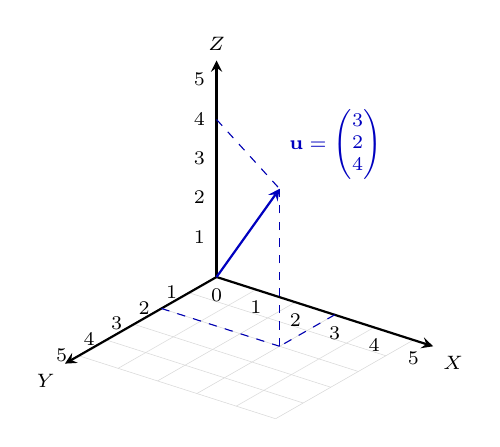
\begin{tikzpicture}[
      >=stealth,
      x={(0.50cm, -0.16cm)},
      y={(-0.35cm, -0.20cm)},
      z={(0cm, 0.50cm)},
      lbl/.style={font=\scriptsize},
      vec3d/.style={thick, ->, blue!75!black},
      dash_blue/.style={dashed, thin, blue!70!black}
    ]
    % Griglia sul piano XY
    \foreach \x in {0,...,5} \draw[lightgray!60, very thin] (\x,0,0) -- (\x,5,0);
    \foreach \y in {0,...,5} \draw[lightgray!60, very thin] (0,\y,0) -- (5,\y,0);

    % Assi 3D
    \draw[thick, ->] (0,0,0) -- (5.5,0,0) node[anchor=north west, lbl] {$X$};
    \draw[thick, ->] (0,0,0) -- (0,5.5,0) node[anchor=north east, lbl] {$Y$};
    \draw[thick, ->] (0,0,0) -- (0,0,5.5) node[anchor=south, lbl] {$Z$};

    % Tacche e numeri
    \foreach \x in {1,...,5} \node[lbl, anchor=north] at (\x,0,-0.05) {\x};
    \foreach \y in {1,...,5} \node[lbl, anchor=east] at (-0.05,\y,0) {\y};
    \foreach \z in {1,...,5} \node[lbl, anchor=east] at (-0.05,0,\z) {\z};
    \node[lbl, anchor=north] at (0,0,-0.05) {0};

    % Proiezioni 3D
    \coordinate (P3D) at (3,2,4);
    \coordinate (Pxy) at (3,2,0);
    \draw[dash_blue] (3,0,0) -- (Pxy) ;
    \draw[dash_blue] (0,2,0) -- (Pxy);
    \draw[dash_blue] (Pxy) -- (P3D) ;
    \draw[dash_blue] (0,0,4) -- (P3D);

    % Vettore e punto P
    \draw[vec3d] (0,0,0) -- (P3D);
    \node[lbl, text=blue!75!black, anchor=south west] at (P3D) {$\mathbf{u} = \begin{pmatrix} 3 \\ 2 \\ 4 \end{pmatrix}$};
  \end{tikzpicture}
\end{minipage}


Di un vettore ci interessa la \textbf{norma}, che non è altro che la "lunghezza" del vettore. La norma di un vettore generico $\underline{x} \in \mathbb{R}^n$ la indichiamo con il simbolo $||\underline{x}||$ e si calcola nel seguente modo 

\[
||\underline{x}|| = \sqrt{x_1^2+x_2^2+ \cdots + x^2_n} = \sqrt{\sum_{i=1}^{n}x_i^2}
\]



Ricordiamo anche le principali proprietà della norma

\begin{teorema}{Proprietà della Norma}{}
  Sia $\underline{x}, \underline{y} \in\mathbb{R}^n$ allora vale 

  
  \begin{itemize}
    \centering
    \item $ ||\underline{x} || = 0 \iff \underline{x} = \underline{0}$
    \item $\forall \lambda \in\mathbb{R}: ||\lambda\underline{x} || = |\lambda|\cdot||\underline{x} ||$
    \item $||\underline{x} + \underline{y} || \leq ||\underline{x}|| + ||\underline{y}|| $
  \end{itemize}
\end{teorema}

Dei vettori possiamo definire le classiche operazioni di somma, sottrazione e moltiplicazione con uno scalare, ora definiamo il prodotto scalare tra due vettori $\underline{x}, \underline{y} \in \mathbb{R}^n$ come 

\[
\underline{x} \cdot \underline{y} = x_1y_1 + x_2y_2 + \cdots x_ny_n = \sum_{i=1}^{n} x_iy_i 
\]

Però si può dimostrare che si può calcolare anche come 
\[
\underline{x} \cdot \underline{y} = ||\underline{x}||||\underline{y}|| \cos\theta
\]

dove $\theta\in\mathbb{R}$ è l'angolo formato tra i due vettori. Con questa nuova espressione per il prodotto scalare, possiamo definire se due vettori sono ortogonali, ovvero quando formano un angolo $\theta=\pi/2$ e che quindi 

\[
\underline{x} \cdot \underline{y} = ||\underline{x}||||\underline{y}|| \cos\dfrac{\pi}{2} = ||\underline{x}||||\underline{y}||  \cdot 0
\]
\[
\underline{x} \cdot \underline{y} = 0
\]



Dalla formula del prodotto scalare possiamo anche trovare una nuova informazione 

\begin{teorema}{Disuguaglianza di Cauchy-Schwarz}{}
  $\forall \underline{x}, \underline{y} \in \mathbb{R}^n$ vale
  \[
  |\underline{x} \cdot \underline{y} | \leq ||\underline{x}|| ||\underline{y}||
  \]
  La saturazione a uguaglianza la abbiamo  
  \[
  |\underline{x} \cdot \underline{y} | = ||\underline{x}|| ||\underline{y}|| \iff \exists \lambda \in\mathbb{R}: \underline{x} = \lambda \underline{y}
  \]
\end{teorema}
\newpage

\section{Elementi di Topologia}

Dopo il breve ripasso sui vettori iniziamo ad aggiungere nuovi elementi, infatti definiamo il concetto di \textbf{palla}

\begin{definizione}{Palla/Disco/Cerchio}{}

  Sia $\underline{p}\in\mathbb{R}^n$ che chiamiamo \textbf{centro} e $r\in\mathbb{R}$ che chiamiamo \textbf{raggio}, definiamo 

  \begin{itemize}
    \item \textbf{Palla Chiusa} come
    \[
    B(\underline{p}, r] = \overline{B(\underline{p}, r)} = \{\underline{x} \in \mathbb{R}^n : ||\underline{x} - \underline{p}|| \leq r\}
    \]
    \item \textbf{Palla Aperta} come
    \[
    B(\underline{p}, r) = \{\underline{x} \in \mathbb{R}^n : ||\underline{x} - \underline{p}|| < r\}
    \]

    \item \textbf{Circonferenza} (o \textbf{Frontiera}) come
    \[
    \partial B(\underline{p}, r) = \{\underline{x} \in \mathbb{R}^n : ||\underline{x} - \underline{p}|| = r\}
    \]
  \end{itemize}

\end{definizione}

Vediamo di capire cosa vuol dire tutto questo, per farlo facciamo l'esempio con $\mathbb{R}^2$.Prendiamo ad esempio $\underline{p} = (2, 3)$ e $r=1$ vediamo questi insiemi cosa rappresentano 

\vspace{0.4cm}

\noindent
% =========================================================
% 1. PALLA CHIUSA (Interno pieno + Bordo continuo)
% =========================================================
\begin{minipage}[t]{0.32\textwidth}
  \centering
  \textbf{\small Palla Chiusa}\\[2pt]
  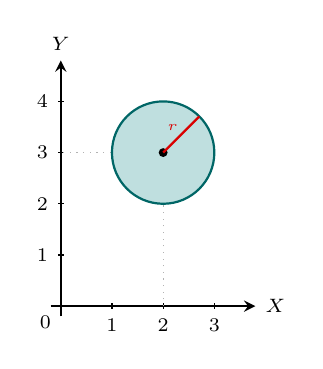
\begin{tikzpicture}[
      >=stealth,
      x=0.65cm, y=0.65cm,
      lbl/.style={font=\scriptsize}
    ]
    % Griglia e assi
    \draw[thick, ->] (-0.2,0) -- (3.8,0) node[anchor=west, lbl] {$X$};
    \draw[thick, ->] (0,-0.2) -- (0,4.8) node[anchor=south, lbl] {$Y$};

    % Tacche
    \foreach \x in {1,2,3} \draw (\x, 0.06) -- (\x, -0.06) node[anchor=north, lbl] {\x};
    \foreach \y in {1,2,3,4} \draw (0.06, \y) -- (-0.06, \y) node[anchor=east, lbl] {\y};
    \node[lbl, anchor=north east] at (0,0) {0};

    % Proiezioni del centro
    \draw[gray!60, dotted] (2,0) -- (2,3) -- (0,3);

    % Disco chiuso: riempimento + linea continua
    \filldraw[fill=teal!25, draw=teal!80!black, thick] (2,3) circle (1);

    % Centro e raggio
    \fill[black] (2,3) circle (1.6pt);
    \draw[-, thick, red!85!black] (2,3) -- ++(45:1) node[midway, above left, font=\tiny, inner sep=1pt] {$r$};
  \end{tikzpicture}
\end{minipage}\hfill
% =========================================================
% 2. PALLA APERTA (Interno pieno + Bordo tratteggiato)
% =========================================================
\begin{minipage}[t]{0.32\textwidth}
  \centering
  \textbf{\small Palla Aperta}\\[2pt]
  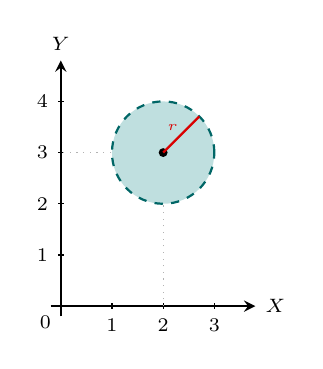
\begin{tikzpicture}[
      >=stealth,
      x=0.65cm, y=0.65cm,
      lbl/.style={font=\scriptsize}
    ]
    % Griglia e assi
    \draw[thick, ->] (-0.2,0) -- (3.8,0) node[anchor=west, lbl] {$X$};
    \draw[thick, ->] (0,-0.2) -- (0,4.8) node[anchor=south, lbl] {$Y$};

    % Tacche
    \foreach \x in {1,2,3} \draw (\x, 0.06) -- (\x, -0.06) node[anchor=north, lbl] {\x};
    \foreach \y in {1,2,3,4} \draw (0.06, \y) -- (-0.06, \y) node[anchor=east, lbl] {\y};
    \node[lbl, anchor=north east] at (0,0) {0};

    % Proiezioni del centro
    \draw[gray!60, dotted] (2,0) -- (2,3) -- (0,3);

    % Disco aperto: riempimento + linea tratteggiata (bordo escluso)
    \fill[teal!25] (2,3) circle (1);
    \draw[teal!80!black, thick, dashed] (2,3) circle (1);

    % Centro e raggio
    \fill[black] (2,3) circle (1.6pt) ;
    \draw[-, thick, red!85!black] (2,3) -- ++(45:1) node[midway, above left, font=\tiny, inner sep=1pt] {$r$};
  \end{tikzpicture}
\end{minipage}\hfill
% =========================================================
% 3. FRONTIERA (Solo la linea continua esterna)
% =========================================================
\begin{minipage}[t]{0.32\textwidth}
  \centering
  \textbf{\small Frontiera}\\[2pt]
  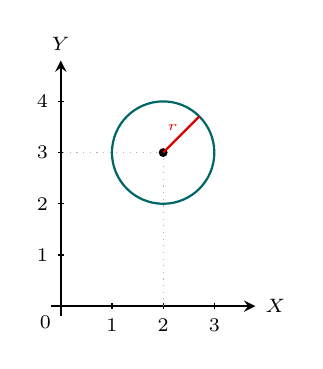
\begin{tikzpicture}[
      >=stealth,
      x=0.65cm, y=0.65cm,
      lbl/.style={font=\scriptsize}
    ]
    % Griglia e assi
    \draw[thick, ->] (-0.2,0) -- (3.8,0) node[anchor=west, lbl] {$X$};
    \draw[thick, ->] (0,-0.2) -- (0,4.8) node[anchor=south, lbl] {$Y$};

    % Tacche
    \foreach \x in {1,2,3} \draw (\x, 0.06) -- (\x, -0.06) node[anchor=north, lbl] {\x};
    \foreach \y in {1,2,3,4} \draw (0.06, \y) -- (-0.06, \y) node[anchor=east, lbl] {\y};
    \node[lbl, anchor=north east] at (0,0) {0};

    % Proiezioni del centro
    \draw[gray!60, dotted] (2,0) -- (2,3) -- (0,3);

    % Frontiera: solo il contorno (interno non colorato)
    \draw[teal!80!black, thick] (2,3) circle (1);

    % Centro e raggio
    \fill[black] (2,3) circle (1.6pt) ;
    \draw[-, thick, red!85!black] (2,3) -- ++(45:1) node[midway, above left, font=\tiny, inner sep=1pt] {$r$};
  \end{tikzpicture}
\end{minipage}

\vspace{0.3cm}

L'idea di palla è lo stesso concetto di un cerchio o sfera portandolo ad una dimensione qualsiasi. Poi la differenza tra le 3 tipologie è che quella aperta contiene solo i punti dentro la palla, la frontiera è solo il "bordo" mentre la palla chiusa è l'unione tra i punti interni e del bordo. Nella terza dimensione la frontiera non è altro che la superficie della sfera, quindi non comprende l'interno della sfera. Allo stesso modo possiamo definire gli ipercubi.

\begin{definizione}{Quadrati/Cubi/Ipercubi}{}

  Sia $\underline{p}\in\mathbb{R}^n$ che chiamiamo \textbf{centro} e $r\in\mathbb{R}$ che chiamiamo \textbf{semi lato}, definiamo 

  \begin{itemize}
    \item \textbf{Ipercubo Chiuso} come
    \[
    Q(\underline{p}, r] = \overline{Q(\underline{p}, r)} = \{\underline{x} \in \mathbb{R}^n : \forall i \leq n \quad |x_i - p_i| \leq r\}
    \]
    \item \textbf{Ipercubo Aperto} come
    \[
    Q(\underline{p}, r) =\{\underline{x} \in \mathbb{R}^n : \forall i \leq n \quad |x_i - p_i| < r\}
    \]
    \item \textbf{Frontiera} come
    \[
    \partial Q(\underline{p}, r) =\{\underline{x} \in \mathbb{R}^n : x_i = p_i \pm r \quad \forall j \ne  i \quad |x_j - p_j| \leq r\}
    \]
  \end{itemize}

\end{definizione}


Per capire come mai questa è la definizione di un ipercubo facciamo l'esempio con $\mathbb{R}^2$, e capiamo cosa rappresenta sul grafico $|x_i - p_i| \leq r$, infatti questo traccia una "striscia" larga $2r$ nella direzione del versore di quella componente. Quindi se prendiamo ad esempio $\underline{p} = (1,1)$ e $r=2$ abbio che le due striscie sono 





\vspace{0.3cm}

\noindent
\begin{minipage}[c]{0.48\textwidth}
  \centering
  \textbf{\small Caso 2D}\\[2pt]
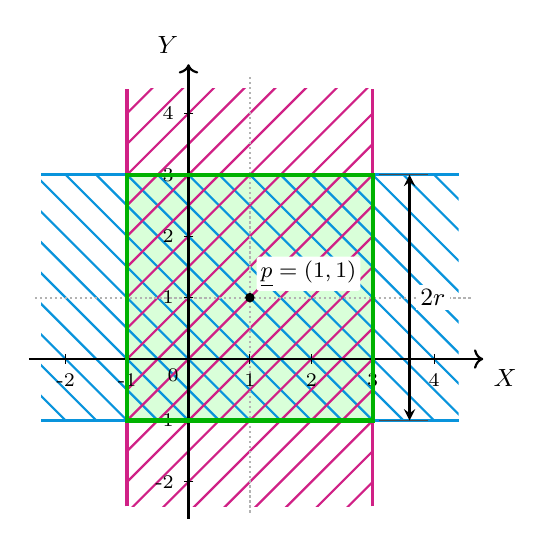
\begin{tikzpicture}[
      scale=0.78,
      lbl/.style={font=\scriptsize},
      title_lbl/.style={font=\small},
      magenta_style/.style={magenta!85!black},
      blue_style/.style={cyan!80!blue},
      green_style/.style={green!70!black}
  ]

  % 1. Sfondo intersezione (quadrato)
  \fill[green!15] (-1, -1) rectangle (3, 3);

  % 2. Tratteggio striscia orizzontale (|y - 1| <= 2)
  \begin{scope}
    \clip (-2.4, -1) rectangle (4.4, 3);
    \foreach \c in {-4, -3.5, ..., 8} {
      \draw[blue_style, thick] (-3, \c + 3) -- (5, \c - 5);
    }
  \end{scope}
  \draw[blue_style, very thick] (-2.4,  3) -- (4.4,  3);
  \draw[blue_style, very thick] (-2.4, -1) -- (4.4, -1);

  % 3. Tratteggio striscia verticale (|x - 1| <= 2)
  \begin{scope}
    \clip (-1, -2.4) rectangle (3, 4.4);
    \foreach \c in {-6, -5.5, ..., 6} {
      \draw[magenta_style, thick] (-2, -2 + \c) -- (4, 4 + \c);
    }
  \end{scope}
  \draw[magenta_style, very thick] (-1, -2.4) -- (-1, 4.4);
  \draw[magenta_style, very thick] ( 3, -2.4) -- ( 3, 4.4);

  % 4. Assi centrati in p = (1, 1)
  \draw[gray!60, densely dotted, thick] (1, -2.5) -- (1, 4.6);
  \draw[gray!60, densely dotted, thick] (-2.5, 1) -- (4.6, 1);

  % 5. Assi cartesiani standard
  \draw[black, thick, ->] (-2.6, 0) -- (4.8, 0) node[anchor=north west, font=\small] {$X$};
  \draw[black, thick, ->] (0, -2.6) -- (0, 4.8) node[anchor=south east, font=\small] {$Y$};

  \foreach \x in {-2, -1, 1, 2, 3, 4}
    \draw (\x, 0.08) -- (\x, -0.08) node[anchor=north, lbl] {\x};
  \foreach \y in {-2, -1, 1, 2, 3, 4}
    \draw (0.08, \y) -- (-0.08, \y) node[anchor=east, lbl] {\y};
  \node[lbl, anchor=north east] at (0, 0) {$0$};

  % 6. Bordo verde
  \draw[green_style, line width=1.6pt] (-1, -1) rectangle (3, 3);

  % 7. Quota 2r
  \draw[black!70, thin] (3.1, -1) -- (3.9, -1);
  \draw[black!70, thin] (3.1,  3) -- (3.9,  3);
  \draw[<->, >=stealth, thick] (3.6, -1) -- (3.6, 3) 
    node[midway, right=2pt, font=\small\bfseries, fill=white, inner sep=1.5pt] {$2r$};

  % 8. Centro p
  \fill[black] (1, 1) circle (2.2pt);
  \node[anchor=south west, font=\footnotesize\bfseries, fill=white, inner sep=1.5pt, rounded corners=1pt] 
    at (1.1, 1.1) {$\underline{p}=(1,1)$};

  \end{tikzpicture}
\end{minipage}\hfill
\begin{minipage}[c]{0.48\textwidth}
  \centering
  \textbf{\small Caso 3D}\\[2pt]
    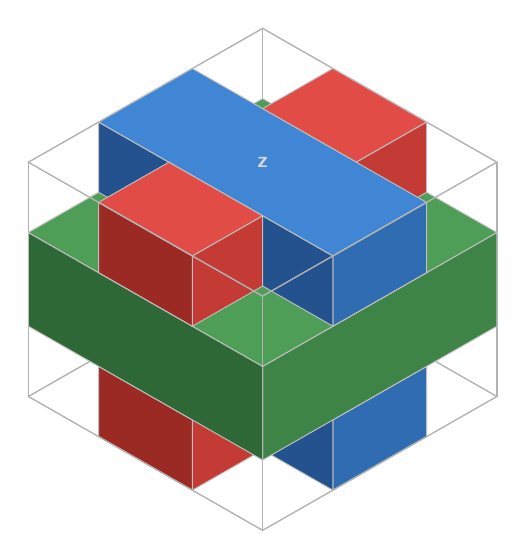
\begin{tikzpicture}[
      % Proiezione assonometrica coerente con la visuale di Desmos 3D
      x={(0.35cm, -0.20cm)},
      y={(-0.35cm, -0.20cm)},
      z={(0cm, 0.35cm)},
      line join=round, 
      line cap=round,
      scale=0.85
  ]

  % Parametri dimensionali
  \def\a{2}  % Semispessore delle regioni: |x|<a, |y|<a, |z|<a
  \def\L{5}  % Limite del volume cubico [-L, L]^3

  % Palette cromatica stile Desmos
  \definecolor{desmosredtop}{RGB}{225, 76, 70}
  \definecolor{desmosredfront}{RGB}{196, 58, 52}
  \definecolor{desmosredside}{RGB}{156, 42, 36}

  \definecolor{desmosbluetop}{RGB}{64, 134, 212}
  \definecolor{desmosbluefront}{RGB}{48, 108, 178}
  \definecolor{desmosblueside}{RGB}{35, 82, 142}

  \definecolor{desmosgreentop}{RGB}{78, 158, 88}
  \definecolor{desmosgreenfront}{RGB}{62, 132, 71}
  \definecolor{desmosgreenside}{RGB}{46, 104, 54}

  \tikzset{
      edge/.style={draw=black!25, line width=0.35pt},
      boxedge/.style={draw=black!30, line width=0.5pt}
  }

  % 1. Spigoli posteriori del cubo
  \draw[boxedge] (-\L, -\L, -\L) -- (-\L, -\L,  \L);
  \draw[boxedge] (-\L, -\L, -\L) -- (-\L,  \L, -\L);
  \draw[boxedge] (-\L, -\L, -\L) -- ( \L, -\L, -\L);
  \draw[boxedge] (-\L,  \L, -\L) -- (-\L,  \L,  \L);
  \draw[boxedge] ( \L, -\L, -\L) -- ( \L, -\L,  \L);
  \draw[boxedge] (-\L, -\L,  \L) -- (-\L,  \L,  \L);
  \draw[boxedge] (-\L, -\L,  \L) -- ( \L, -\L,  \L);

  % 2. Blocchi inferiori visibili (z in [-L, -a])
  \filldraw[fill=desmosbluefront, edge] (\L, -\a, -\L) -- (\L, \a, -\L) -- (\L, \a, -\a) -- (\L, -\a, -\a) -- cycle;
  \filldraw[fill=desmosblueside,  edge] (-\L, \a, -\L) -- (\L, \a, -\L) -- (\L, \a, -\a) -- (-\L, \a, -\a) -- cycle;

  \filldraw[fill=desmosredfront, edge] (\a, \a, -\L) -- (\a, \L, -\L) -- (\a, \L, -\a) -- (\a, \a, -\a) -- cycle;
  \filldraw[fill=desmosredside,  edge] (-\a, \L, -\L) -- (\a, \L, -\L) -- (\a, \L, -\a) -- (-\a, \L, -\a) -- cycle;

  % 3. Piastra Verde orizzontale (|z| < 2)
  \filldraw[fill=desmosgreenfront, edge] (\L, -\L, -\a) -- (\L, \L, -\a) -- (\L, \L, \a) -- (\L, -\L, \a) -- cycle;
  \filldraw[fill=desmosgreenside,  edge] (-\L, \L, -\a) -- (\L, \L, -\a) -- (\L, \L, \a) -- (-\L, \L, \a) -- cycle;
  \filldraw[fill=desmosgreentop,   edge] (-\L, -\L, \a) -- (\L, -\L, \a) -- (\L, \L, \a) -- (-\L, \L, \a) -- cycle;

  % 4. Blocchi superiori visibili (z in [a, L])
  \filldraw[fill=desmosredtop,   edge] (-\a, -\L, \L) -- (\a, -\L, \L) -- (\a, -\a, \L) -- (-\a, -\a, \L) -- cycle;
  \filldraw[fill=desmosredfront, edge] (\a, -\L, \a)  -- (\a, -\a, \a)  -- (\a, -\a, \L)  -- (\a, -\L, \L)  -- cycle;

  \filldraw[fill=desmosbluefront, edge] (\L, -\a, \a) -- (\L, \a, \a) -- (\L, \a, \L) -- (\L, -\a, \L) -- cycle;
  \filldraw[fill=desmosblueside,  edge] (-\L, \a, \a) -- (\L, \a, \a) -- (\L, \a, \L) -- (-\L, \a, \L) -- cycle;
  \filldraw[fill=desmosbluetop,   edge] (-\L, -\a, \L) -- (\L, -\a, \L) -- (\L, \a, \L) -- (-\L, \a, \L) -- cycle;

  \filldraw[fill=desmosredfront, edge] (\a, \a, \a) -- (\a, \L, \a) -- (\a, \L, \L) -- (\a, \a, \L) -- cycle;
  \filldraw[fill=desmosredside,  edge] (-\a, \L, \a) -- (\a, \L, \a) -- (\a, \L, \L) -- (-\a, \L, \L) -- cycle;
  \filldraw[fill=desmosredtop,   edge] (-\a, \a, \L) -- (\a, \a, \L) -- (\a, \L, \L) -- (-\a, \L, \L) -- cycle;

  % Etichetta asse Z
  \node[font=\bfseries\sffamily\footnotesize, text=white!85!black] at (0, 0, \L) {z};

  % 5. Spigoli anteriori del cubo
  \draw[boxedge] ( \L, -\L, -\L) -- ( \L,  \L, -\L) -- (-\L,  \L, -\L);
  \draw[boxedge] ( \L,  \L, -\L) -- ( \L,  \L,  \L);
  \draw[boxedge] ( \L, -\L,  \L) -- ( \L,  \L,  \L) -- (-\L,  \L,  \L);

  \end{tikzpicture}





\end{minipage}

\vspace{0.3cm}
Quindi dovete immaginarvi questi fasci di rette che passano per $\underline{p}$ e larghe $2r$ e che la loro intersezione forma il vero e proprio ipercubo. In 3d la visualizazione diventa ancora più complessa, infatti nello spazio non abbiamo delle semplici fascie (come nel 2d) ma abbiamo dei "muri" larghi $2r$.

Per la frontiera sembra più complicato di quanto non lo sia veramente. Per capirla pensiamo al cubo in 3d perchè a due dimensioni non diventa chiaro. La frontiera è la superficie del cubo e quindi sono le 6 faccie del cubo, quindi ogni quadrato avrà due coppie di equazioni della forma $|x_j-p_j|\leq r$. Prendiamo una delle faccie qualsiasi, e pensiamo che dal centro una delle 3 coordinate dista $\pm r$ mentre le altre coordinate formano un quadrato. Quindi per ogni coordinata fissiamo $x_i=p_i\pm r$ e le altre coordninate formano un quadrato $|x_j - p_j|\leq r$. 



\begin{teorema}{}{}
  Ogni palla è inclusa in un quadrato con lo stesso centro e viceversa, in particolare 

\[
  B(\underline{p}, r] \subseteq Q(\underline{p}, r] \subseteq B(\underline{p}, \sqrt{n}r]
\]

\end{teorema}

\begin{proof}
 Iniziamo dimostrando che 

  \[
    B(\underbar{p}, r]  \subseteq Q(\underbar{p}, r] 
  \]


  Dalla definizione di palle sappiamo che vale 
  \[
  \sqrt{(x_1-p_1)^2+(x_2-p_2)^2+\cdots + (x_n-p_n)^2} \leq r
  \]

  Ora prendiamo un qualsiasi componente del vettore: $x_i$ e notiamo che vale 

  \[
  \forall i \leq n \qquad |x_i-p_i| \leq    \sqrt{(x_1-p_1)^2+(x_2-p_2)^2+\cdots + (x_n-p_n)^2} 
  \]
  Da cui
  \[
  \forall i \leq n \qquad  |x_i-p_i| \leq   r
  \]

  Riconosciamo che questa è la definizione proprio di $Q(\underbar{p}, r] $. Ora invede dobbiamo dimostrare che 

  \[
    Q(\underbar{p}, r]  \subseteq B(\underbar{p}, \sqrt{n}r] 
  \]

  Partiamo dalla definizione di ipercubo

  \[
   \forall i \leq n \qquad  |x_i-p_i| \leq   r
  \]

  Ma se eleviamo tutto al quadrato abbiamo 


  \[
   \forall i \leq n \qquad  (x_i-p_i)^2 \leq   r^2
  \]

  Da cui 

  \begin{align*}
    (x_1-p_1)^2+(x_2-p_2)^2+\cdots + (x_n-p_n)^2   &\leq   r^2 +r^2 +\cdots + r^2 \\
    &= nr^2 
  \end{align*}
  
  

  Dato che entrambe le quantità sono positive possiamo applicare la radice quadrata ambo i membri

  \[
   \sqrt{(x_1-p_1)^2+(x_2-p_2)^2+\cdots + (x_n-p_n)^2}  \leq   \sqrt{n}r 
  \]

  Ma questa è la definizione di $B(\underbar{p}, \sqrt{n}r] $.

  


\end{proof}

\newpage
\begin{definizione}{Intorno di un punto}{}
  
  Sia $\underline{p}\in \mathbb{R}^n$, $U \subseteq \mathbb{R}^n$ allora diciamo che $U$ è \textbf{intorno} di $\underline{p}$ se 

  \[
  \exists \delta > 0: \quad B(\underline{p}, \delta] \subseteq U
  \]
\end{definizione}


Vediamo di capire facendo un disegno generico, $U$ è la regione  a righe
\begin{center}
  
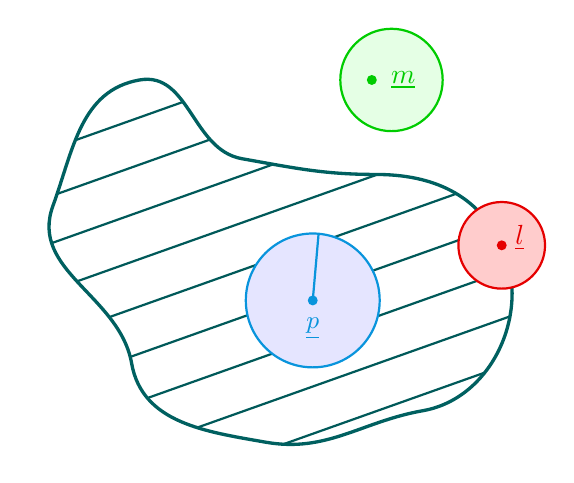
\begin{tikzpicture}[
    >=stealth,
    lbl/.style={font=\small},
    curve_style/.style={teal!75!black, very thick},
    hatch_style/.style={teal!70!black, thick},
    blue_ball/.style={draw=cyan!80!blue, fill=blue!10, thick},
    ext_ball/.style={draw=green!80!black, fill=green!10, thick},
    bnd_ball/.style={draw=red!90!black, fill=red!20, thick}
  ]

  % Definiering av den godtyckliga slutna kurvan för U
  \def\curveU{
    (-2.5, 0.2) to[out=70, in=190] 
    (-1.4, 1.8) to[out=10, in=170] 
    (-0.1, 0.8) to[out=-10, in=180] 
    (1.6, 0.6) to[out=0, in=115] 
    (3.2, -0.3) to[out=-65, in=10] 
    (2.2, -2.4) to[out=190, in=-10] 
    (0.2, -2.8) to[out=170, in=-80] 
    (-1.5, -1.8) to[out=100, in=-110] 
    cycle
  }

  % 1. Skraffering (diagonala linjer) inuti U
  \begin{scope}
    \clip \curveU;
    \foreach \y in {-5, -4.4, ..., 3.5} {
      \draw[hatch_style] (-4, \y) -- (5, \y + 3.2);
    }
  \end{scope}

  % 2. Randen för området U
  \draw[curve_style] \curveU;


  % 3. Inre punkt p och dess öppna boll B(p, r) helt inuti U
  \coordinate (P) at (0.8, -1.0);
  \filldraw[blue_ball] (P) circle (0.85);
  \draw[cyan!80!blue, thick] (P) -- ++(85:0.85);
  \fill[cyan!80!blue] (P) circle (1.8pt);
  \node[cyan!80!blue, lbl, anchor=north] at (0.8, -1.1) {$\underline{p}$};

  % 4. Yttre punkt m och dess boll disjunkt från U
  \coordinate (M) at (1.8, 1.8);
  \filldraw[ext_ball] (M) circle (0.65);
  \fill[green!80!black] (1.55, 1.8) circle (1.8pt);
  \node[green!80!black, lbl, font=\bfseries] at (1.95, 1.8) {$\underline{m}$};

  % 5. Randpunkt l med en boll som skär både det inre och det yttre
  \coordinate (L) at (3.2, -0.3);
  \filldraw[bnd_ball] (L) circle (0.55);
  \fill[red!90!black] (L) circle (1.8pt);
  \node[red!90!black, lbl, font=\bfseries, anchor=west] at (3.25, -0.2) {$\underline{l}$};

\end{tikzpicture}
\end{center}


In questo disegno, $U$ è intorno solamente di $\underline{p}$, perchè è l'unico punto che se iniziamo a disegnare una palla rientra completamente nella regione $U$. Mentre il vettore $\underline{m}$ è facile vedere che non può avere $U$ come intorno dato che basta disegnare una palla sufficientemente piccola e  non apparterrà mai a $U$. Quello meno intuito forse è il vettore $\underline{l}$, perchè qualsiasi palla noi scegliamo avremo una porzione all'interno di $U$ e una porzione fuori da $U$, ma proprio perchè abbiamo anche una piccola porzione esterna da $U$ per qualsiasi palla noi scegliamo, allora per forza $U$ non è intorno di $\underline{l}$.



\begin{definizione}{Punto Interno/Esterno/Frontiera}{}
  Sia $\underline{p},\underline{m},\underline{l}\in \mathbb{R}^n$, $U \subseteq \mathbb{R}^n$ allora diciamo che 
  \begin{itemize}
    \item $\underline{p}$ è \textbf{punto interno} a $U$ se $U$ è intorno di $\underline{p}$
    \item $\underline{m}$ è \textbf{punto esterno} a $U$ se $\mathbb{R}^n\setminus U$ è intorno di $\underline{m}$
    \item $\underline{l}$ è \textbf{punto di frontiera} a $U$ se 
    \[
    \forall \delta > 0: \quad B(\underline{l}, \delta] \cap U \neq \varnothing\,\, \land \,\, B(\underline{l}, \delta] \setminus U \neq \varnothing
    \]
  \end{itemize}
\end{definizione}


Penso che il concetto di punto esterno ed interno sia abbastanza comprensibile ai più. Quello che invece è da discutere è sicuramente il punto di frontiera, querchè un punto di frontiera è un qualsiasi punto che indipendentemente da che cerchio gli si crea intorno avrà sempre una porzione sulla regione di $U$ e uno al di fuori, e questo sempre. Quindi si può pensare che tutti i punti sul "bordo" siano punti di frontiera, e infatti è così. In più è indipendette se il punto fa parte dell'insieme $U$. Però i punti di frontiera non sono solo quelli "al bordo" ma sono anche i punti "isolati" e i "buchi".  Facciamo un esempio pratico e definiamo

\[
U = \{((x,y) \in \mathbb{R}^2 : \,\, (x-1)^2+y^2\leq 4 \,\,\land\,\, x>1)\} \cup \{(-1,0)\} \setminus \{(2,0)\}
\]


Nel piano cartesiano la regione $U$

\begin{center}
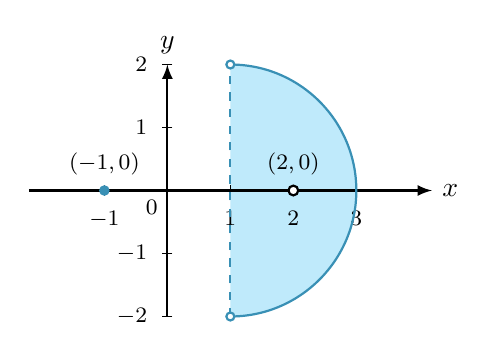
\begin{tikzpicture}[>=latex, scale=0.80]

  % 1. Riempimento del semidisco destro centrato in (1,0) di raggio 2
  \fill[cyan!25] (1, -2) arc (-90:90:2) -- cycle;

  % 2. Assi cartesiani
  \draw[->, thick] (-2.2, 0) -- (4.2, 0) node[right] {$x$};
  \draw[->, thick] (0, -2) -- (0, 2) node[above] {$y$};

  % Tacche e valori numerici sugli assi
  \foreach \x in {-1, 1, 2, 3}
    \draw (\x, 0.08) -- (\x, -0.08) node[below=2pt, font=\footnotesize] {$\x$};
  \foreach \y in {-2, -1, 1, 2}
    \draw (0.08, \y) -- (-0.08, \y) node[left=2pt, font=\footnotesize] {$\y$};
  \node[below left, font=\footnotesize] at (0,0) {$0$};

  % 3. Bordo circolare esterno (x-1)^2 + y^2 = 4 per x >= 1 (INCLUSO -> continuo)
  \draw[thick, cyan!70!black] (1, -2) arc (-90:90:2);

  % 4. Bordo verticale x = 1 per y in [-2, 2] (ESCLUSO -> tratteggiato)
  \draw[thick, dashed, cyan!70!black] (1, -2) -- (1, 2);

  % Estremi del segmento (1, 2) e (1, -2) esclusi (cerchietti vuoti)
  \filldraw[fill=white, draw=cyan!70!black, thick] (1,  2) circle (1.8pt);
  \filldraw[fill=white, draw=cyan!70!black, thick] (1, -2) circle (1.8pt);

  % 5. Punto rimosso (2,0) (ESCLUSO -> buco vuoto con bordo)
  \filldraw[fill=white, draw=black, thick] (2, 0) circle (2.2pt);
  \node[above=2pt, font=\footnotesize] at (2, 0) {$(2,0)$};

  % 6. Punto isolato (-1,0) (INCLUSO -> punto pieno nero)
  \fill[cyan!70!black] (-1, 0) circle (2.4pt);
  \node[above=2pt, font=\footnotesize] at (-1, 0) {$(-1,0)$};

\end{tikzpicture}  
\end{center}

Dalla definizione che abbiamo dato, possiamo riconoscere che tutta il perimetro del semicerchio sono punti di frontiera, e questo non cambia se il perimetro è compreso (come per la semicircoferenza) oppure no (come per la retta $x=1$) nell'insieme $U$. Poi ci sono anche i punti $(-1,0)$ e $(2,0)$ che son da discutere, infatti prendiamo il punto $(-1,0)$, se noi disegnamo un qualsiasi cerchio attorno a lui vedremmo che

\[
B((-1,0), \delta] \nsubseteq \mathbb{R}^n\setminus U
\]

Questo perchè $(-1,0) \in B((-1,0), \delta]$ mentre nel nostro dominio $(-1,0) \notin \mathbb{R}^n\setminus U$ prioprio perchè $(-1,0) \in U$. Di conseguenza $ \mathbb{R}^n\setminus U$ non è intorno di $(-1,0)$ e di conseguenza $(-1,0)$ non può essere un punto isolato. Però non può nemmeno essere un punto interno, dato che preso qualsiasi palla con centro $(-1,0)$ ci sono sempre dei punti di $\mathbb{R}^n\setminus U$, e quindi non può essere nemmeno un punto interno, e di conseguenza $(-1, 0)$ è un punto di frontiera. Ragionamento analogo per il punto $(2,0)$, solo che il ragionamento è al contrario dato che $(2,0) \notin U$. 



\begin{definizione}{Interno/Esterno/Frontiera/Chiusura di $U$}{}
  Sia $U\subseteq\mathbb{R}^n$, definiamo 
  \begin{center}
    
  \begin{itemize}
    \item \textbf{Interno} di $U$:  
    $
    \text{Int }U = U^0 = \{\underline{x}\in\mathbb{R}^n: \; x \text{ è interno a } U\}
    $
    \item \textbf{Esterno} di $U$: 
    $
    \text{Ext }U  = \{\underline{x}\in\mathbb{R}^n: \; x \text{ è esterno a } U\}
    $
    \item \textbf{Frontiera} di $U$:  
    $
    \partial U  = \{\underline{x}\in\mathbb{R}^n: \; x \text{ è frontiera di } U\}
    $
    \item \textbf{Chiusura} (o \textit{Closure}) di $U$: 
    $
   \bar{U}  = \text{Clos}(U) = U \cup \partial U
    $
  \end{itemize} 
  \end{center}
\end{definizione}

Di questi insieme non sono altro che l'insieme dei punti che abbiamo definito prima. L'unico nuovo è la chiusura che non è altro che l'aggiunta della frontiera (ovvero del "bordo") all'insieme originale.

\begin{definizione}{Insiemi Aperti e Chiusi}{}
  Sia $U\subseteq\mathbb{R}^n$, diciamo che 


  \begin{center}    
  \begin{itemize}
    \item $U$ è \textbf{aperto} se $U = U^0$
    \item $U$ è \textbf{chiuso} se $\mathbb{R}^n\setminus U$ è aperto
  \end{itemize}
\end{center}

  \end{definizione}


  \section{Curve Parametriche}

  \begin{definizione}{Curva Parametrica}{}
    Siano $\gamma_1, \gamma_2, \cdots, \gamma_n: D\subseteq\mathbb{R} \to \mathbb{R}$ funzioni tali che $\gamma_i \in C^0(D)$ allora definiamo una \textbf{curva parametrica} $\gamma: D\to \mathbb{R}^n$ come
    \[
    \underline{\gamma}(t) = (\gamma_1(t)\, , \, \gamma_2(t)\, ,\, \dots \, ,\, \gamma_n(t) )
    \]  
  \end{definizione}


  Il concetto fondamentale è che le curve parametriche sono \textbf{funzioni} e non vanno confuse con la loro immagine!

  \begin{definizione}{Immagine/Sostegno/Supporto di una curva}{}
    Sia $\underline{\gamma}: D\to \mathbb{R}^n$ una curva parametrica, $I \subseteq D$,  definiamo \textbf{l'immagine} di $\gamma$ nell'intervallo $I$ come 
    \[
    \text{Im}(\underline{\gamma}, I) = \{\underline{\gamma}(t): \forall t \in I\} 
    \]
  \end{definizione}

  Fondamentale distinguere che una curva è una funzione, mentre la sua immagine è l'insieme dei punti che genera la funzione, e che quindi se parliamo di funzioni 2d e 3d, allora l'immagina è il grafico che disegnamo. Vediamo quindi un esempio di come disegnarla, prendiamo la seguente curva nel suo dominio $[0, 2\pi]$
  
  \[
  \underline{\gamma}(t) = \begin{pmatrix}
    16\sin^3(t) \\
    13\cos t -5\cos 2t -2\cos 3t -cos 4t
  \end{pmatrix}
  \]

  Per disegnarla basta prendere tutti i valori di $t$ nel suo dominio e segnare i punti sul grafico, in questo caso il grafico della funzione 
\begin{center}
  
  \begin{tikzpicture}[scale=0.16]
  % Assi cartesiani (opzionali)
  \draw[->, black] (-20,0) -- (20,0) node[right] {$x$};
  \draw[->, black] (0,-20) -- (0,16) node[above] {$y$};

  % Curva parametrica
  \draw[red, thick, smooth, samples=360, domain=0:360, variable=\t]
    plot ({16*sin(\t)*sin(\t)*sin(\t)},
          {13*cos(\t) - 5*cos(2*\t) - 2*cos(3*\t) - cos(4*\t)}) -- cycle;
      \node[anchor=north east] at (17,14.5) {$\underline{\gamma}(t)$};
\end{tikzpicture}
\end{center}

\textbf{N.B.} Una curva può avere più immagini, a seconda del dominio. Ad esempio se prendiamo la curva $\underline{\gamma}(t) = (\cos t, \sin t)$, se la definiamo con il dominio $D = [0, 2\pi]$ l'immagine sarà cerchio unitario, mentre se scegliamo il dominio $D=[0, \pi]$ l'immagine sarà una semicircoferenza. Questo è un esempio che a parità di curva possiamo avere più immagini, dipendentemente dalla scelta del dominio. Funziona anche il contrario però, infatti un'immagine può essere fatta da più curve, infatti se prendiamo sempre il cerchio unitario che abbiamo nominato prima, possiamo disegnarlo anche con la curva $\underline{\gamma}(t)=(\cos 2t, -\sin 2t)$ con $D=[0, \pi]$.


\begin{definizione}{Vettore Velocità e Vettore Accelerazione}{}
  Sia $\underline{\gamma}: D \to \mathbb{R}^n$ una curva parametrica tale che $\gamma_i \in C^1(D)$ allora definiamo
\begin{itemize}
  \item Il \textbf{vettore velocità} come 
  \[
  \underline{\dot{\gamma}}(t) =  (\dot{\gamma}_1(t)\, , \, \dot{\gamma}_2(t)\, ,\, \dots \, ,\, \dot{\gamma}_n(t) )
  \]
\end{itemize}

Inoltre se $\gamma_i \in C^2(D)$ allora possiamo definire anche 
\begin{itemize}
  \item Il \textbf{vettore accelerazione} come 
  \[
  \underline{\ddot{\gamma}}(t) =  (\ddot{\gamma}_1(t)\, , \, \ddot{\gamma}_2(t)\, ,\, \dots \, ,\, \ddot{\gamma}_n(t) )
  \]
\end{itemize}

\end{definizione}


Chiaramente questi concetti si rifanno molto al concetto di velocità e accelerazione che abbiamo già incontrato in fisica, quindi non serve spendere molte altre parole. Con il vettore velocità possiamo trovare la retta tangente alla funzione per un certo $t\in D$ come eravamo abituati con analsi 1

\[
r: \{\underline{\gamma}(t) + \underline{\dot{\gamma}}(t)(s-t): \, \forall s \in \mathbb{R}\}
\]

In realtà come abbiamo già studiato ad analisi 1, la retta tangente non è altro che lo sviluppo di Taylor ai primi 2 termini, pertanto possiamo fare lo sviluppo di Taylor anche della nostra curva gamma 

\[
T_{t_0}[\underline{\gamma}] = \underline{\gamma}(t_0) + \underline{\dot{\gamma}}(t_0)(t-t_0)+ \dfrac{1}{2}\underline{\ddot{\gamma}}(t_0)(t-t_0)^2 +  \dfrac{1}{3!}\underline{\dddot{\gamma}}(t_0)(t-t_0)^3 + \cdots = \sum_{n=0}^{+\infty} \dfrac{1}{n!} \underline{\gamma}^{(n)}(t_0) (t-t_0)^n
\]

\begin{definizione}{Curva Piana/Chiusa/Semplice/Regolare}{}
  Sia  $\underline{\gamma}: D \subseteq \mathbb{R}\to \mathbb{R}^n$ una curva parametrica, allora diciamo che 
  \begin{itemize}
    \item $\underline{\gamma}$ è \textbf{piana} se $\text{Im}(\underline{\gamma}, D)$ giace su un un piano 
    \item $\underline{\gamma}$ è \textbf{chiusa} se il dominio è della forma $D=[a,b]$ e vale
    \[
    \underline{\gamma}(a) = \underline{\gamma}(b)  
    \]
    \item $\underline{\gamma}$ è \textbf{semplice} se $\underline{\gamma}$ è iniettiva, ad eccezion fatta che se la curva è anche chiusa non continiamo il caso $\underline{\gamma}(a)=\underline{\gamma}(b)$.
    \item $\underline{\gamma}$ è \textbf{regolare} in $I\subseteq D^0$ se $\underline{\gamma} \in C^1(I)$
    \[
      \underline{\dot{\gamma}}(t) \ne \underline{0} \quad \forall t \in I
    \]
  \end{itemize}
\end{definizione}

\newpage
Andiamo ora a vedere dei casi particolari per capire bene questi consetti 

\vspace{0.2cm}
\begin{minipage}{0.24\textwidth}
    \centering
    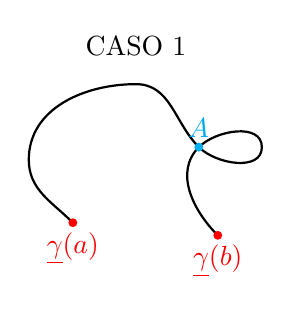
\begin{tikzpicture}[scale=0.8]
        \node at (0.5, 2.8) {CASO 1};
        
        % Curva Caso 1
        \draw[thick] (-0.5, 0)
            to[out=135, in=-90] (-1.2, 1)
            to[out=90, in=180] (0.5, 2.2)
            to[out=0, in=135] (1.5, 1.2)
            to[out=-45, in=-90] (2.5, 1.2)
            to[out=90, in=45] (1.5, 1.2)
            to[out=-135, in=135] (1.8, -0.2);
            
        % Punti ed etichette
        \fill[red] (-0.5,0) circle (2pt) node[below] {$\underline{\gamma}(a)$};
        \fill[red] (1.8,-0.2) circle (2pt) node[below] {$\underline{\gamma}(b)$};
        \fill[cyan] (1.5,1.2) circle (2pt) node[above, cyan] {$A$};
    \end{tikzpicture}
\end{minipage}\hfill
\begin{minipage}{0.24\textwidth}
    \centering
    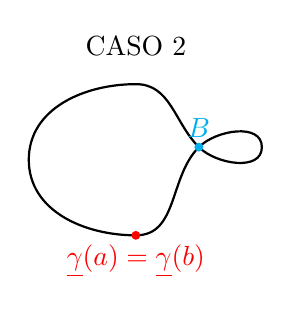
\begin{tikzpicture}[scale=0.8]
        \node at (0.5, 2.8) {CASO 2};
        
        % Curva Caso 2
        \draw[thick] (0.5, -0.2)
            to[out=180, in=-90] (-1.2, 1)
            to[out=90, in=180] (0.5, 2.2)
            to[out=0, in=135] (1.5, 1.2)
            to[out=-45, in=-90] (2.5, 1.2)
            to[out=90, in=45] (1.5, 1.2)
            to[out=-135, in=0] (0.5, -0.2);
            
        % Punti ed etichette
        \fill[red] (0.5,-0.2) circle (2pt) node[below] {$\underline{\gamma}(a)=\underline{\gamma}(b)$};
        \fill[cyan] (1.5,1.2) circle (2pt) node[above, cyan] {$B$};
    \end{tikzpicture}
\end{minipage}\hfill
\begin{minipage}{0.24\textwidth}
    \centering
    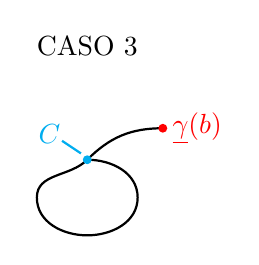
\begin{tikzpicture}[scale=0.8]
        \node at (1, 2.8) {CASO 3};
        
        % Curva Caso 3
        \draw[thick](1, 1)
            to[out=0, in=90] (1.8, 0.4)
            to[out=-90, in=0] (1, -0.2)
            to[out=180, in=-90] (0.2, 0.4)
            to[out=90, in=225] (1, 1)
            to[out=45, in=180] (2.2, 1.5);
            
        % Punti ed etichette
        \fill[red] (2.2,1.5) circle (2pt) node[right] {$\underline{\gamma}(b)$};
        \fill[cyan] (1,1) circle (2pt);
        \draw[cyan, thick] (0.6, 1.3) -- (0.9, 1.1);
        \node[cyan] at (0.4, 1.4) {$C$};
    \end{tikzpicture}
\end{minipage}\hfill
\begin{minipage}{0.24\textwidth}
    \centering
    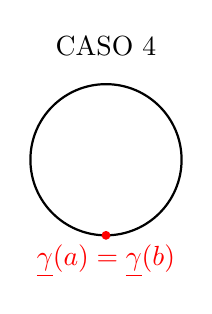
\begin{tikzpicture}[scale=0.8]
        \node at (0, 2.8) {CASO 4};
        
        % Curva Caso 4 (Cerchio)
        \draw[thick] (0, 1) circle (1.2);
        
        % Punti ed etichette
        \fill[red] (0, -0.2) circle (2pt) node[below] {$\underline{\gamma}(a)=\underline{\gamma}(b)$};
    \end{tikzpicture}
\end{minipage}
\vspace{0.2cm}


Il caso 1 si può notare sicuramente che non è chiusa dato che $\underline{\gamma}(a)\ne \underline{\gamma}(b) $ e in più non è nemmeno regolare, perchè la curva passa due volte per il punto $A$. 

Il caso 2 invece è una curva chiusa proprio perchè l'inizio e la fine conincidono, mentre non è regolare, questo perchè oltre al punto di inizio/fine (che questo è tollerato per la definizione di regolare) c'è anche il punto $B$ che viene visitato due volte, e questo è sufficiente per rendere la curva non regolare. 

Il caso 3 si può notare subito che non è regolare sempre per via del punto $C$, e soppratutto non è chiusa perche il punto di inizio (che coindice con $\underline{\gamma}(a) = C$) è diverso da  $\underline{\gamma}(b) $. 

Infine il caso 4 possiamo dire con sicurezza che è chiuso, ma non siamo sicuri che sia regolare questo perchè non sappiamo quanti "giri" ha fatto, infatti se supponiamo per semplicità che $\underline{\gamma}(t) = (\cos t, \sin t)$ e scegliamo $D=[0, 2\pi]$ allora sarebbe anche regolare, invece se scegliamo un dominio $D=[0, 4\pi]$ avremmo che la circonferenza sarebbe disegnata due volte e di conseguenza non sarebbe iniettiva perchè per ogni punto dell'immagine abbiamo 2 punti del dominio che la generano. Questo discorso in realtà lo possiamo fare anche per tutti gli altri casi, perchè nessuno ha assicurato che per disegnare quelle curve non siamo "tornati indietro", che in quel caso invaliderebbe la regolarità. Quindi diciamo che la regolarità non è assicurata guardando solamente il grafico. 

\begin{definizione}{Lunghezza della Curva}{}
 Sia  $\underline{\gamma}: D \subseteq \mathbb{R}\to \mathbb{R}^n$ una curva parametrica tale che $\underline{\gamma(t)} \in C^1(D)$, sia $[a, b]\subseteq D$, definiamo come \textbf{lunghezza della curva $\underline{\gamma}$ nell'intervallo} $[a, b]$ come 

 \[
 L(\underline{\gamma}, [a, b]) = \int_{a}^{b} ||\underline{\dot{\gamma}}(t)|| dt
 \]
\end{definizione}

L'idea di questa definizione riprende proprio il concetto si spazio in fisica, infatti in fisica se abbiamo la legge della velocità, possiamo calcolare quanto spazio viene percorso in un periodo di tempo usiamo la stessa definizione. 
L'unica differenza che essendo una curva a più dimensioni, prendiamo il suo modulo che altro non è che la velocità a cui sta andando istante per istante. Interessante è il caso a una variabile, ovvero prendiamo una funzione generica $f:\mathbb{R}\to\mathbb{R}$ allora possiamo parametrizzarla con una curva nel seguente modo $\underline{\gamma}(t) = (t, f(t))$, da cui $\underline{\dot{\gamma}}(t) = (1, \dot{f}(t))$ e quindi preso un generico intervallo $[a, b]$ abbiamo che la lunghezza della curva è 
\[
L = \int_{a}^{b}\sqrt{1+[\dot{f}(t)]^2} dt
\]

\end{document}

